\documentclass{beamer}
\usepackage{amssymb}
\setbeamertemplate{navigation symbols}{}
\setbeamertemplate{footline}[page number]
\usepackage{amsmath}
\usepackage{amsrefs}
\usepackage{graphicx}
\usepackage{bookman}
\usepackage{url}
\usepackage{amsthm}
\usepackage{verbatim}
\usepackage{xcolor}
\bibliographystyle{amsmath}
\usetheme{Madrid}
\usecolortheme{dolphin}
\useoutertheme[footline=authortitle]{miniframes}

%\newtheorem{theorem}{Theorem}[section]
%\newtheorem{corollary}[theorem]{Corollary}

\title[]{Early Evaluation of IBM BlueGene/P}
\author[]{Tyler Allen\\ \footnotesize Clemson University}

\begin{document}

%\setbeamercolor{title}
\begin{frame}
\begin{center}
\maketitle
\end{center}
\end{frame}

\begin{frame}{Outline}
Today we will:
\begin{itemize}
\item Discuss IBM's BlueGene/P Architecture
\item Discuss the specifications of the hardware
\item Examine benchmarks from a BlueGene/P implementation
\end{itemize}
\end{frame}

\section{Background}
\subsection{Background}
\begin{frame}{Early Evaluation}
\begin{itemize}
\item Goal: Evaluate performance of architecture
\item Several metrics:
\begin{itemize}
\item Hardware and Topology Specifications
\item Microbenchmarks and Kernels
\item Target Applications
\end{itemize}
\end{itemize}
\end{frame}

\begin{frame}{BlueGene/P Architecture}
\begin{itemize}
\item Developed by IBM
\item Second Generation Architecture
\item Successor to BlueGene/L
\item Early Evaluation of IBM BlueGene/P by S. Alam et al. in 2008
\item Authors from Oak Ridge National Laboratory
\end{itemize}
\end{frame}


\section{Specifications}
\subsection{Nodes}
\begin{frame}{System on Chip}
\begin{itemize}
\item Four PowerPC $450$ cores at $850$ MHz
\item $3.4$ GFlop/s per core
\item On-chip routing and network protocols
\item Low power consumption: $1.8$ watts per GFlop/s
\end{itemize}
\end{frame}

\begin{frame}{Nodes}
\begin{itemize}
\item $2$GB shared RAM per node, soldered
\item $13.6$ GFlop/s per node
\item Connections to $5$ networks
\item $32$K L1 Cache
\item $14$ Stream Prefetching L2
\item $8$MB Shared L3
\end{itemize}
\end{frame}


\begin{frame}{Racks}
\begin{itemize}
\item $4096$ cores per rack
\item Standard cooling
\item Cores per Rack far exceeds prior architectures
\item Possible because of low power consumption
\item $72$ Racks give $1$ PFLOP/s
\end{itemize}
\end{frame}

\begin{frame}{Racks}
\begin{figure}
\begin{center}
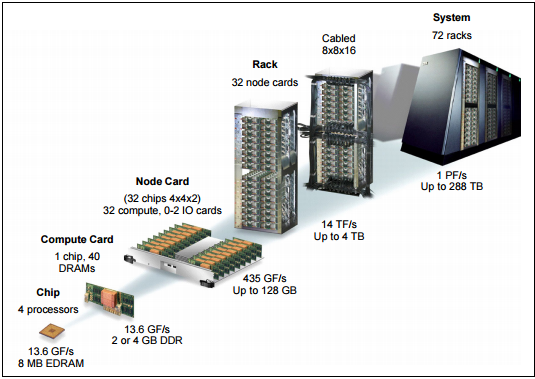
\includegraphics[scale=0.5]{figs/racks.png}
\caption{Image from IBM Redbook \cite{ibm}}
\end{center}
\end{figure}
\end{frame}

\subsection{Topology}
\begin{frame}{Topology}
\begin{itemize}
\item $3$-D Torus Topology
\item Global Collective Tree (Global Broadcasts)
\item $10$ Gigabit Ethernet (IO)
    \begin{itemize}
        \item IO requests route through Global Collective Tree
    \end{itemize}
\item Global interrupt network
\item JTAG control network
\end{itemize}
\end{frame}

\subsection{Specifications and Hardware}
\begin{frame}{Comparison to BlueGene/L}
\begin{center}
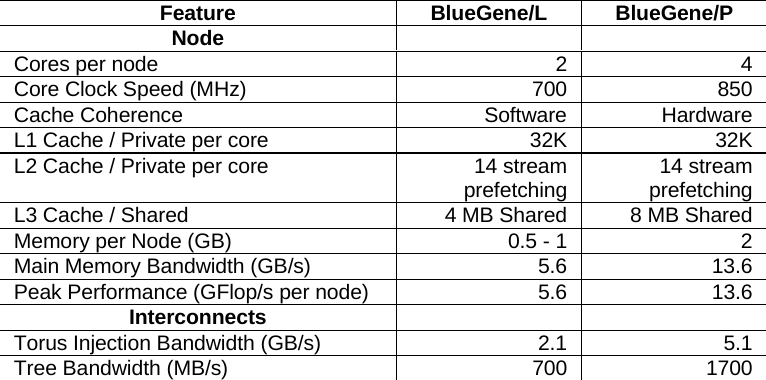
\includegraphics[scale=0.5]{figs/sysconfig.png}
\end{center}
\end{frame}

\begin{frame}{Node Hardware}
\begin{figure}
\begin{center}
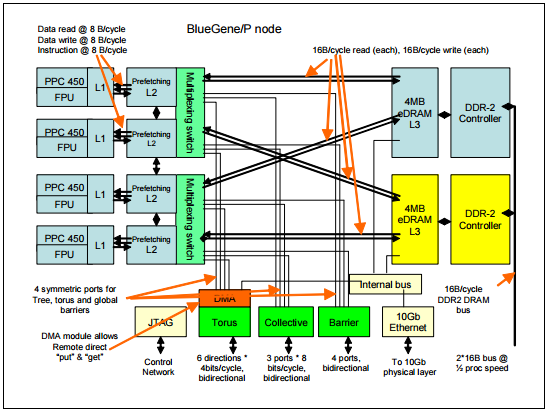
\includegraphics[scale=0.5]{figs/computenode.png}
\caption{Image from IBM Redbook \cite{ibm}}
\end{center}
\end{figure}
\end{frame}

\begin{frame}{Node Modes}
\begin{itemize}
\item Nodes can be used in different modes:
\begin{itemize}
    \item Symmetric Multiprocessor mode - $1$ MPI Task, $4$ threads each
    \item Dual Node mode - $2$ MPI Tasks, $2$ threads each
    \item Virtual Node mode - $4$ MPI Tasks, $1$ thread each
\end{itemize}
\end{itemize}
\end{frame}

\section{Benchmarks}
\begin{frame}{Benchmarks Overview}
\begin{itemize}
\item Several types of benchmarks
\begin{itemize}
\item HPCC Challenge Kernels - single/parallel performance
\item Halo Benchmark - Network and Communication
\item MPI Collective - MPI performance
\item Target Scientific Applications - Architecture Purpose
\end{itemize}
\end{itemize}
\end{frame}

\begin{frame}{Benchmarks}
We will look at an implementation of BG/P at Argonne National lab, Intrepid.
\begin{itemize}
\item Intrepid is IBM standard configuration.
\item Intrepid has $40$ racks.  
\item We will compare Intrepid to the Cray XT system at ORNL.
\end{itemize}
\end{frame}

\begin{frame}{Cray XT Comparison}
\begin{center}
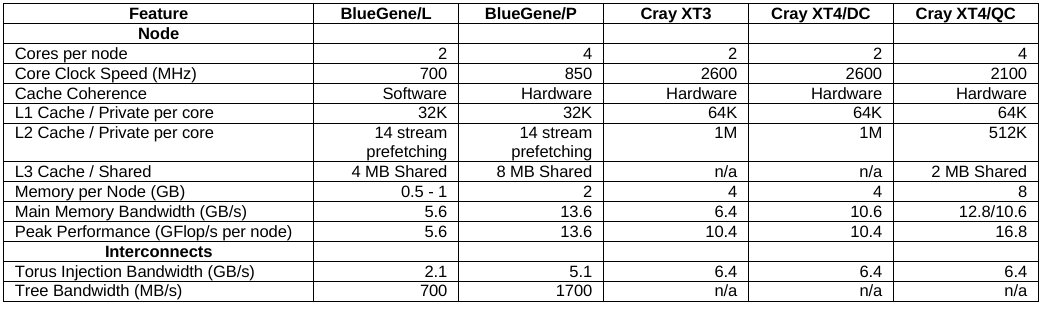
\includegraphics[scale=0.33]{figs/xt.png}
\end{center}
\end{frame}

\subsection{Microbenchmarks and Kernels}
\begin{frame}{HPCC Performance Table}
\begin{figure}
\begin{center}
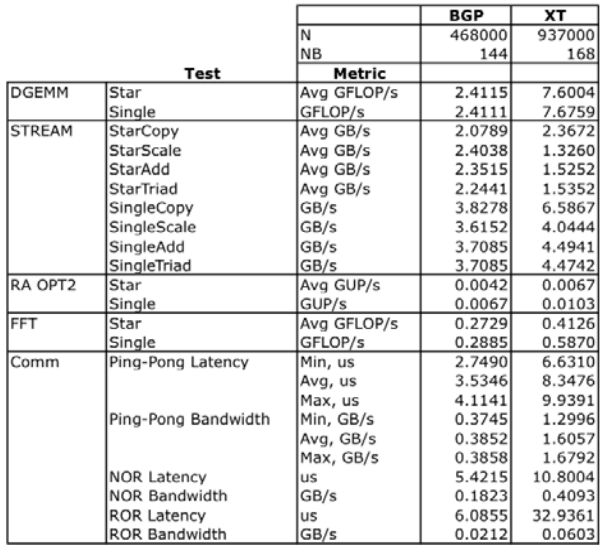
\includegraphics[scale=0.33]{figs/single.png}
\caption{Results of Single Processor and Embarrassingly Parallel Tests, as well as
communication tests.}
\end{center}
\end{figure}
\end{frame}

\begin{frame}{HPCC Performance}
\begin{figure}
\begin{center}
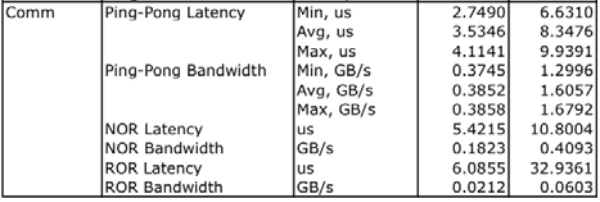
\includegraphics[scale=0.7]{figs/hpcc1.png}
\end{center}
\end{figure}
\end{frame}

\begin{frame}{Single Process, Embarassingly Parallel, Communication}
\begin{itemize}
\item BG/P does not perform as well on single process/embarassingly parallel
tests. Why?
\item BG/P has a lower clock rate than Cray XT
\item Cray XT also has more memory
\item Cray XT also has larger problem size to compensate
\item BG/P is strong when latency is low
\end{itemize}
\end{frame}

\begin{frame}{Parallel Tests}
\begin{figure}
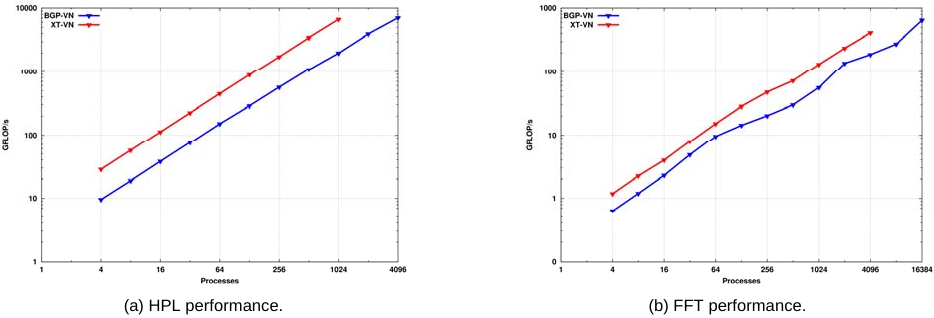
\includegraphics[scale=0.45]{figs/parallel1.png}
\caption{Similar scaling. XT has higher clock rate, larger problem size.}
\end{figure}
\end{frame}

\begin{frame}{Parallel Tests}
\begin{figure}
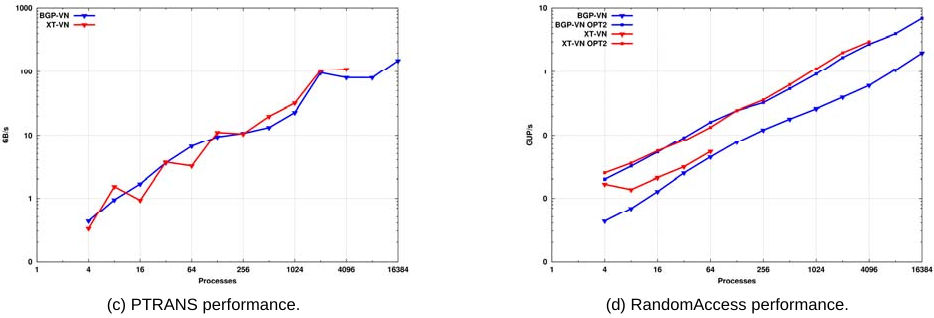
\includegraphics[scale=0.45]{figs/parallel2.png}
\caption{Similar scaling. XT has higher clock rate, larger problem size.}
\end{figure}
\end{frame}

\subsection{Communication}
\begin{frame}
\begin{itemize}
\item Communication benchmarks determine how different network parameters
effect performance.
\item Three parameters for Halo Benchmarks:
\begin{itemize}
\item MPI Protocols
\item Process Mapping
\item Grid Selection
\item Identifies communication strengths/weaknesses
\end{itemize}
\end{itemize}
\end{frame}

\begin{frame}{Halo Benchmark: MPI Protocols}
\begin{figure}
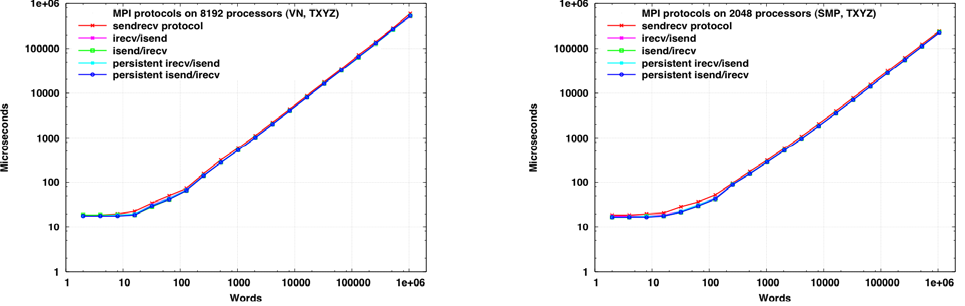
\includegraphics[scale=0.45]{figs/halo1.png}
\caption{MPI Protocol is largely unimportant.}
\end{figure}
\end{frame}

\begin{frame}{Halo Benchmark: Process Mappings}
\begin{figure}
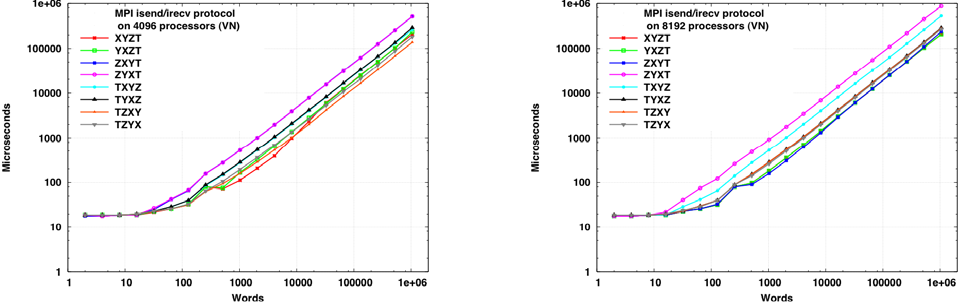
\includegraphics[scale=0.45]{figs/halo2.png}
\caption{Mapping is unimportant for low volumes, but is important as size grows.}
\end{figure}
\end{frame}

\begin{frame}{Halo Benchmark: Grid Size}
\begin{figure}
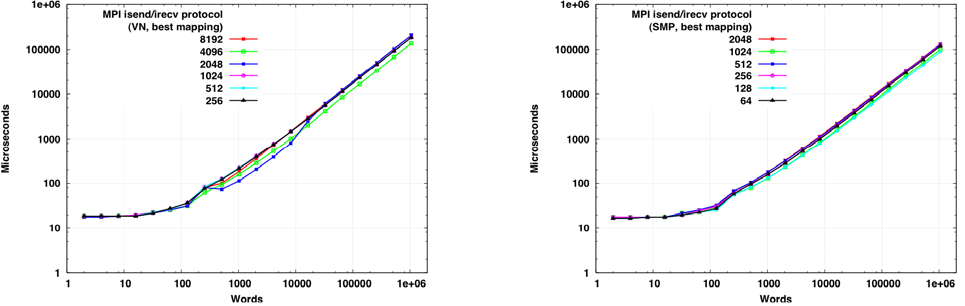
\includegraphics[scale=0.45]{figs/halo3.png}
\caption{Performance is largely unrelated to processor grid size.}
\end{figure}
\end{frame}

\begin{frame}{MPI Collective}
\begin{itemize}
\item MPI Collective emphasises latency as problem sizes grow.
\item Tests performance with MPI\_SUM operation.
\begin{itemize}
\item MPI\_SUM reduces float values to a single value.
\item Modified version included to add double precision.
\end{itemize}
\item B\_CAST, a broadcast function, is also tested.
\end{itemize}
\end{frame}

\begin{frame}{MPI Collective Performance}
\begin{figure}
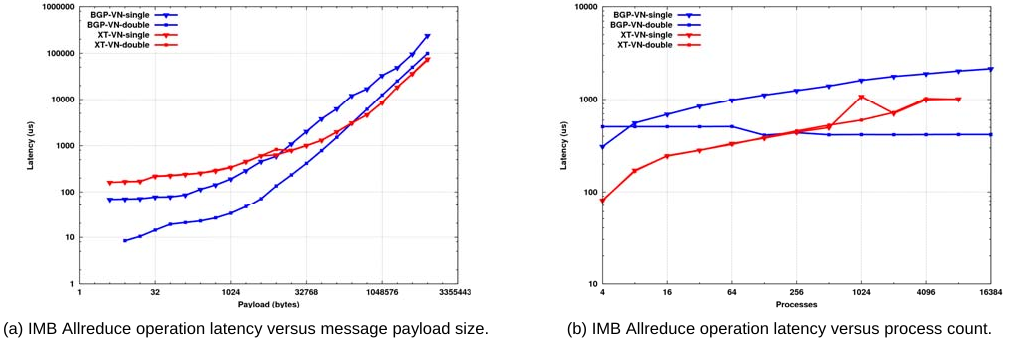
\includegraphics[scale=0.40]{figs/mpi1.png}
\caption{BG/P scales better than XT with double precision values.}
\end{figure}
\end{frame}

\begin{frame}{MPI Collective Performance}
\begin{figure}
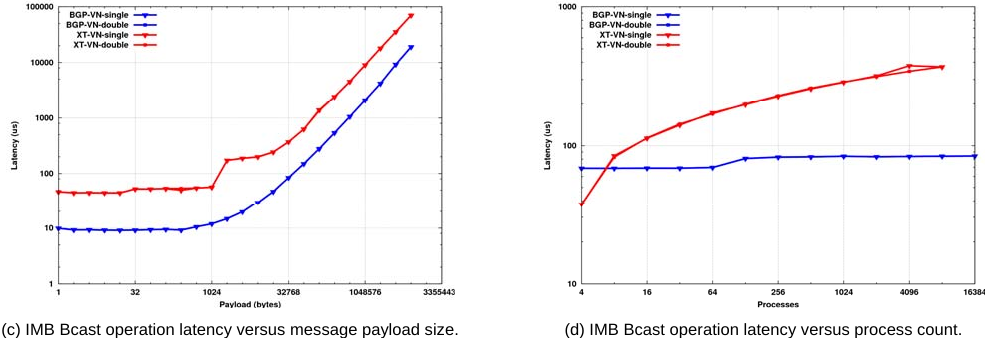
\includegraphics[scale=0.42]{figs/mpi2.png}
\caption{BG/P scales better than XT thanks to Global Collective Tree.}
\end{figure}
\end{frame}

\subsection{TOP$500$ HPL}
\begin{frame}{TOP$500$}
\begin{itemize}
\item With Linpack HPL Benchmark, BG/P ranked $74$ on June $2008$ TOP$500$.
\item Ranked $5^{th}$ overall on on Green500.
\end{itemize}
\end{frame}




\subsection{Applications}
\begin{frame}{Sample Applications}
\begin{itemize}
\item Several Department of Energy applications were used as benchmarks.
\item Applications represent target domain of BG/P
\item Performance in these applications is higher priority than individual
metrics.
\end{itemize}
\end{frame}

\begin{frame}{Sample Applications}
\begin{itemize}
\item BG/P is competitive at tasks with high communication cost.
\item One example is the Parallel Ocean Program with load imbalances.
\end{itemize}
\begin{center}
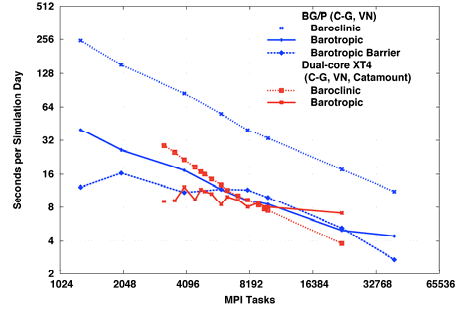
\includegraphics[scale=.45]{figs/pop.png}
\end{center}
\end{frame}

\begin{frame}{Sample Applications cont.}
\begin{itemize}
\item Some applications do not perform as well on BG/P
\item The Community Atmospheric Model (CAM) is one example.
\item Issues with CAM's performance are currently inherent to the program.
\end{itemize}
\begin{center}
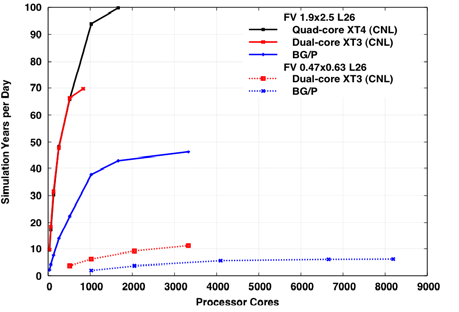
\includegraphics[scale=.45]{figs/cam.png}
\end{center}
\end{frame}

\section{Power}
\begin{frame}{Power Consumption}
\begin{center}
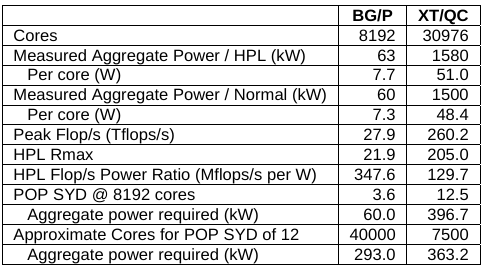
\includegraphics[scale=.45]{figs/power.png}
\end{center}
\begin{itemize}
\item Power consumption is very low on BP/G
\item Power consumption/performance can be low for scientific computing.
\end{itemize}
\end{frame}


\section{Conclusion}
\begin{frame}{Summary}
\begin{itemize}
\item BG/P is an IBM Supercomputer Architecture
\item BG/P shows good performance in low latency conditions.
\item BG/P scales for most applications.
\item BG/P also has low power consumption.
\item For some tasks, BG/P may have much lower performance.
\item BG/P has very low power usage compared to other clusters for most applications.
\end{itemize}
\end{frame}

\begin{frame}{References}
\bibliography{project.bib}
\nocite{*}
\end{frame}

\end{document}
